\documentclass[12pt]{article} % Clase de documento, tamaño de letra 12pt

% Paquetes importantes
\usepackage[utf8]{inputenc}   % Codificación de entrada UTF-8 para caracteres acentuados
\usepackage[T1]{fontenc}      % Codificación de salida para que el texto se vea bien en PDF
\usepackage[spanish]{babel}   % Traduce términos automáticos al español (ej. "Figura", "Resumen")

\usepackage{csquotes}         % Recomendado para manejar comillas y citas con biblatex
\usepackage{graphicx}         % Permite incluir imágenes con \includegraphics
\usepackage{setspace}         % Para controlar interlineado; APA pide interlineado doble
\usepackage{geometry}         % Controla los márgenes de la página (APA pide 1 pulgada = 2.54cm)
\usepackage[hidelinks]{hyperref}        % Habilita enlaces clicables en el PDF (tabla de contenido, referencias)
\usepackage[style=apa, backend=biber]{biblatex}  % Bibliografía con estilo APA 7 y gestor biber
\addbibresource{referencias.bib}  % Archivo con las referencias bibliográficas (formato .bib)

% Carga tu paquete personalizado que contiene el comando \imprimircaratula
\usepackage{caratula}

%para decorar el indice
\usepackage{tocloft} %Conectar los títulos con los números de página usando puntos
\renewcommand{\cftsecleader}{\cftdotfill{\cftdotsep}} %Esto añadirá los "........" entre el título y la página.
\setcounter{tocdepth}{4}   % incluye paragraph en la ToC
\setcounter{secnumdepth}{4}% (opcional) numera hasta paragraph

% Define los márgenes recomendados por APA: 1 pulgada en todos lados
\geometry{letterpaper, margin=1in}

% Permite personalizar el formato de títulos (secciones y subsecciones)
\usepackage{titlesec}
% Define estilo para títulos de sección: tamaño grande y negrita
\titleformat{\section}{\normalfont\large\bfseries}{\thesection}{1em}{}
% Define estilo para títulos de subsección: tamaño normal y negrita
\titleformat{\subsection}{\normalfont\normalsize\bfseries}{\thesubsection}{1em}{}

% Define interlineado doble, que es requerido por APA
\doublespacing

%para la tabla
\usepackage{pdflscape} %Para rotar la página
\usepackage{adjustbox} %Para redimensionar automáticamente el contenido
\usepackage{tabularx} %Para hacer que la tabla ocupe todo el ancho de la página usando columnas flexibles
\usepackage{array} % Para usar >{\centering\arraybackslash}
\usepackage[table,xcdraw]{xcolor} %Para darle color al encabezado
\definecolor{headerbg}{HTML}{D9E1F2} % Para definir un color de encabezado
\usepackage{multirow}      % Para combinar filas

%para personalizar el header
\usepackage{fancyhdr}           % Para encabezados y pies personalizados
\pagestyle{fancy}               % Activar fancyhdr para todas las páginas
\fancyhf{}                      % Limpia encabezados y pies por defecto
\fancyhead[L]{J. Aulla; M. Millan} % Encabezado a la izquierda con las siglas
\fancyhead[R]{\thepage}
\renewcommand{\headrulewidth}{0pt} %quita la linea debajo de los nombres y numero de pagina

%para anexo
\usepackage{tocloft}
\usepackage{float}

%espaciado
%\usepackage{setspace}
%\doublespacing  % interlineado doble
\setlength{\parskip}{1em}







% Datos para título, autor y fecha (aunque no se usan porque tienes portada personalizada)
\title{Título del Documento en Formato APA 7}
\author{Nombre del Autor}
\date{\today}

%-----------------------------------------------------------------------------------
%inicio del documento
%-----------------------------------------------------------------------------------



\begin{document}

% Imprime la portada con el comando definido en tu paquete caratula.sty
\imprimircaratula
\newpage

\section*{Diagrama de Caso de USO}

\begin{figure}[H]
    \centering
    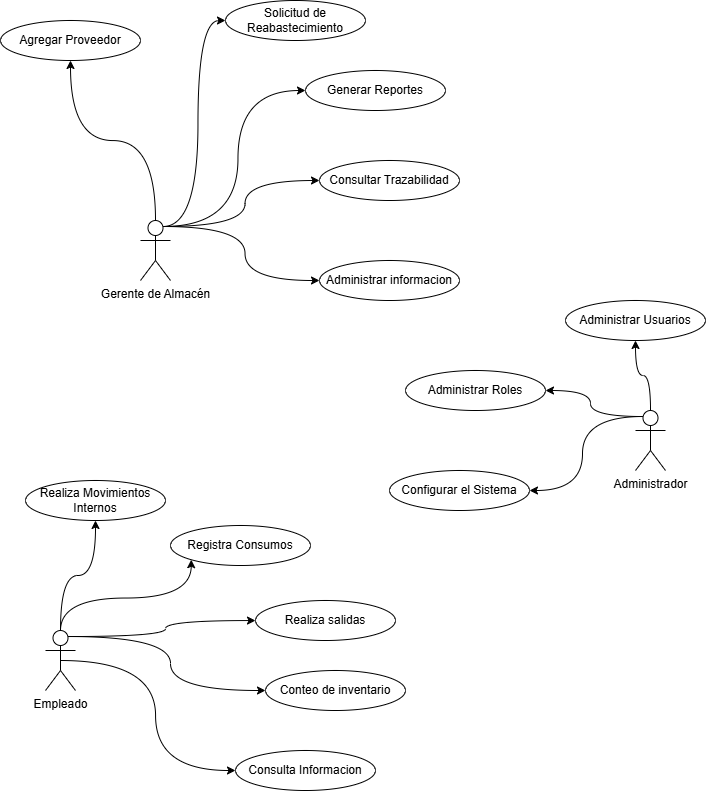
\includegraphics[width=1\textwidth]{caso uso integrador1.png}
    \label{fig:imagen_ejemplo} % Etiqueta para referenciar la imagen en texto
\end{figure}

\section*{Diagrama de Secuencia}
\subsection*{Administrador}

\begin{figure}[H]
    \centering
    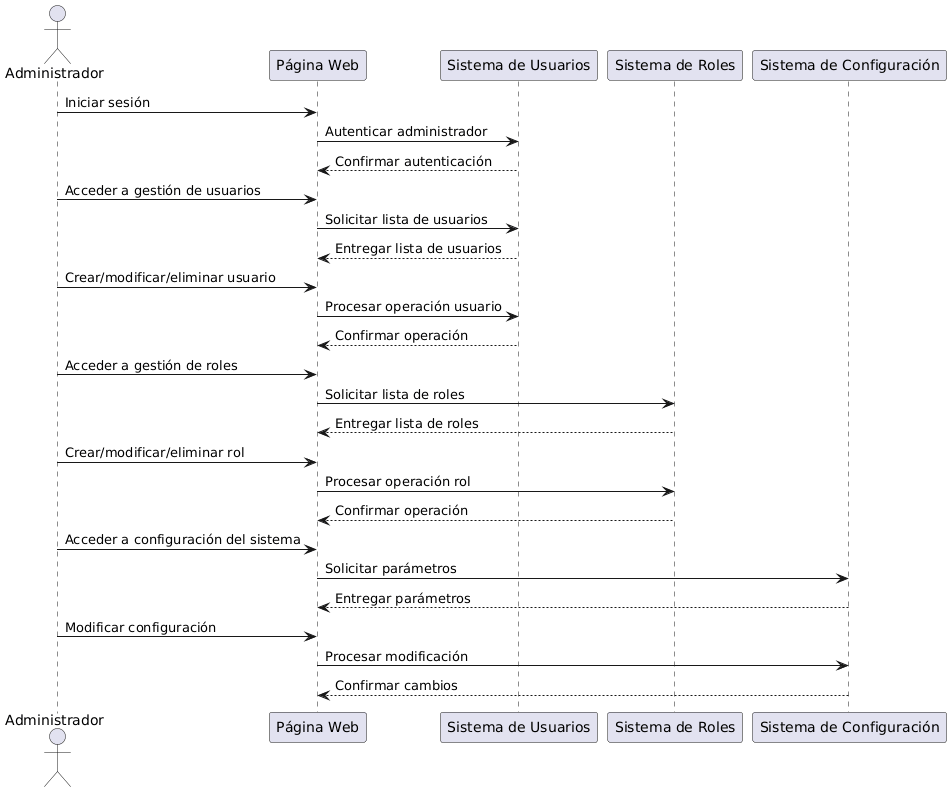
\includegraphics[width=1\textwidth]{administrador.png}
    \label{fig:imagen_ejemplo} % Etiqueta para referenciar la imagen en texto
\end{figure}

\subsection*{Gerente de Almacén}

\begin{figure}[H]
    \centering
    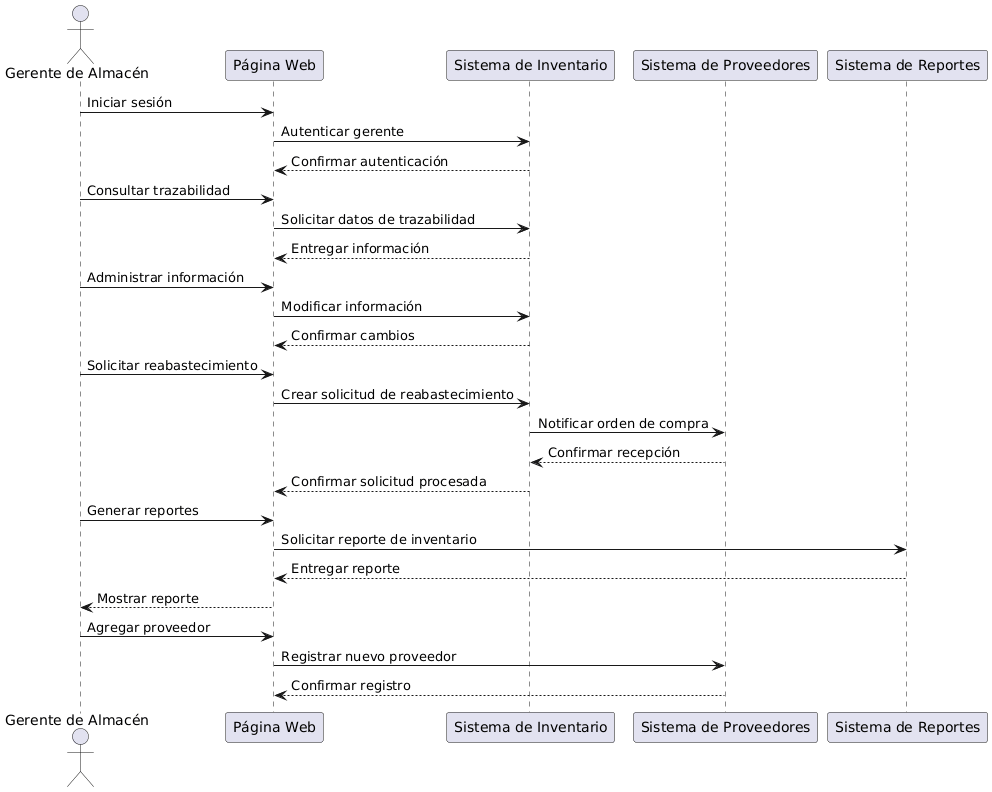
\includegraphics[width=1\textwidth]{gerente.png}
    \label{fig:imagen_ejemplo} % Etiqueta para referenciar la imagen en texto
\end{figure}

\subsection*{Empleado}

\begin{figure}[H]
    \centering
    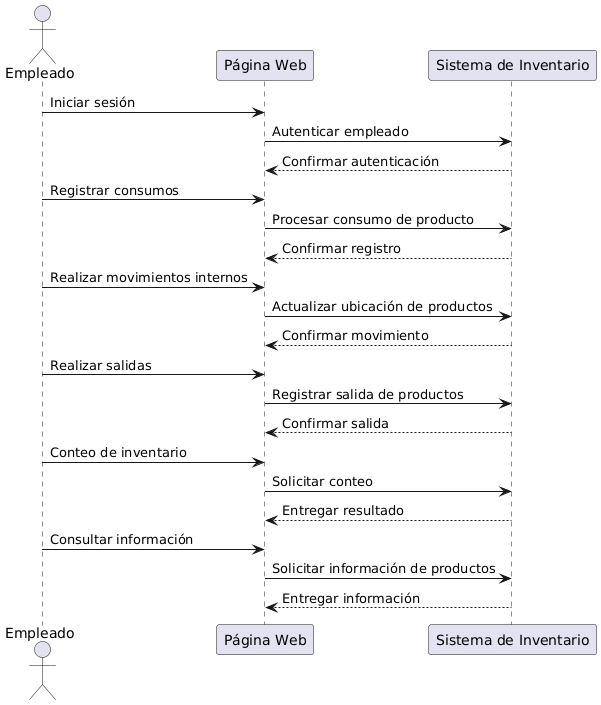
\includegraphics[width=1\textwidth]{empleado.png}
    \label{fig:imagen_ejemplo} % Etiqueta para referenciar la imagen en texto
\end{figure}

\end{document}
